\chapter{Từ cơ học hạt đến các trường cổ điển}

\section{Trường là gì}

Trong bài giảng trước, ta đã xây dựng cơ học hạt tương đối tính từ một tác dụng bất biến. Bây giờ ta thay đổi đối tượng động lực học. Chủ đề ở đây là lý thuyết trường cổ điển, không phải lý thuyết trường lượng tử. Cơ học lượng tử đôi khi sẽ cung cấp một phép so sánh hữu ích, nhưng các phương trình trong chương này mô tả các trường cổ điển thông thường. Điện từ học là mô hình quen thuộc làm nền ở đây: sóng điện từ lan truyền trong không gian và tương tác với các hạt mang điện. Ta bắt đầu với một trường còn đơn giản hơn nữa.

Một không-thời gian có thể có nhiều tọa độ không gian, nhưng nó có một tọa độ thời gian. Viết
\begin{equation}
x^\mu=(t,x^1,\ldots,x^d),
\end{equation}
trong đó chỉ số không gian \(i=1,\ldots,d\). Số \(d\) có thể là ba, như trong thế giới của chúng ta, hoặc một, hai, chín, hai mươi lăm, hay bất kỳ số nào khác hữu ích trong một mô hình. Điều bất đối xứng quan trọng ở giai đoạn này là vẫn chỉ có một hướng thời gian. Bài giảng này không cố giải thích vì sao các lý thuyết có nhiều thời gian lại khó đến vậy; nó chỉ đơn giản chấp nhận khuôn khổ chỉ có một thời gian, trong đó vật lý nhân quả thông thường được phát biểu.

Trường là một đại lượng đo được mà giá trị của nó có thể thay đổi từ điểm này sang điểm khác và từ lúc này sang lúc khác. Nhiệt độ là một ví dụ đơn giản:
\begin{equation}
T=T(\mathbf{x},t).
\end{equation}
Nó gán một số cho mỗi sự kiện, nên nó là một trường vô hướng. Vận tốc gió cũng biến thiên theo không gian và thời gian, nhưng nó có độ lớn và hướng, do đó có nhiều thành phần; nó là một trường vectơ. Trong vật lý tương đối tính, các vectơ tự nhiên có bốn thành phần chứ không phải ba.

Trong phần lớn bài giảng này, trường chỉ có một thành phần và được ký hiệu bằng chữ cái Hy Lạp tương ứng với \(f\):
\begin{equation}
\phi=\phi(\mathbf{x},t).
\label{eq:sr4-field-definition}
\end{equation}
Về sau, việc gọi \(\phi\) là một vô hướng sẽ có ý nghĩa nhiều hơn là chỉ nói rằng nó có một thành phần. Nó sẽ có nghĩa là mọi quan sát viên quán tính đều gán cùng một giá trị cho \(\phi\) tại cùng một sự kiện vật lý. Quy luật biến đổi đó chỉ được đưa vào sau khi cơ học biến phân đã được xây dựng.

\section{Nguyên mẫu hạt}

\subsection{Một tọa độ được gọi là \texorpdfstring{\(\phi\)}{phi}}

Con đường nhanh nhất đến lý thuyết trường bắt đầu bằng việc lùi lại xét một hạt phi tương đối tính thông thường. Hãy cho hạt chuyển động trên một đường thẳng, nhưng gọi tọa độ của nó là \(\phi\) thay vì \(x\). Về mặt toán học không có gì bắt buộc phải gọi một tọa độ là \(x\); cái tên khác thường này được chọn để làm rõ phép tương tự sắp xuất hiện. Hãy vẽ thời gian theo phương ngang. Khi đó toàn bộ lịch sử của hạt là một đường cong \(\phi(t)\), có thể đi qua cả các giá trị dương lẫn âm.

Với các thời điểm đầu và cuối cố định \(a\) và \(b\), tác dụng là
\begin{align}
A[\phi]
&=\int_a^b dt\,L(\phi,\dot\phi),\\
L(\phi,\dot\phi)
&=\frac{m}{2}\dot\phi^{\,2}-V(\phi).
\label{eq:sr4-particle-lagrangian}
\end{align}
Phương trình Euler--Lagrange là
\begin{equation}
\frac{d}{dt}\left(\frac{\partial L}{\partial\dot\phi}\right)
-\frac{\partial L}{\partial\phi}=0.
\label{eq:sr4-particle-el}
\end{equation}
Đối với Lagrangian trong \eqref{eq:sr4-particle-lagrangian},
\begin{equation}
\frac{\partial L}{\partial\dot\phi}=m\dot\phi,
\qquad
\frac{\partial L}{\partial\phi}=-\frac{dV}{d\phi},
\end{equation}
nên
\begin{equation}
\boxed{m\ddot\phi=-\frac{dV}{d\phi}}.
\label{eq:sr4-newton}
\end{equation}
Đây đơn giản là phương trình Newton, được viết với \(\phi\) làm tọa độ.

\begin{figure}[htbp]
\centering
\includegraphics[width=0.90\textwidth]{lecture_04_figure_01.png}
\caption{Phương trình Euler--Lagrange thông thường và kết quả Newton tương ứng của nó cho tọa độ \(\phi(t)\).}
\lectureframe{00:10:18}
\end{figure}

Đường đi vật lý làm cho tác dụng dừng trong khi hai đầu mút được giữ cố định. Bài giảng thường nói \emph{cực tiểu}, nhưng phát biểu chính xác là tính dừng: đường đi có thể cho một cực tiểu, một cực đại, hoặc một giá trị dừng khác. Một mô hình trực giác hữu ích là chia khoảng thời gian thành nhiều đoạn nhỏ. Khi đó tác dụng trở thành một hàm của nhiều giá trị lấy mẫu của \(\phi\). Dịch chuyển các giá trị ấy, trong khi vẫn giữ cố định hai đầu mút, rồi lấy đạo hàm theo từng giá trị của chúng là tiền thân hữu hạn chiều của phương trình Euler--Lagrange.

\subsection{Cơ học như một lý thuyết trong \texorpdfstring{\(0+1\)}{0+1} chiều}

Bây giờ hãy tưởng tượng một thế giới có thời gian nhưng không có chiều không gian nào. Không gian của nó là một điểm duy nhất. Một trường trong thế giới ấy không thể phụ thuộc vào vị trí, vì không có vị trí nào để nó phụ thuộc vào; nó chỉ có thể là một hàm \(\phi(t)\). Vì thế, cơ học hạt thông thường với một tọa độ có thể được hiểu như một lý thuyết trường trong \(0+1\) chiều. Toán học không hề thay đổi. Chỉ có cách diễn giải thay đổi, từ vị trí của một hạt sang giá trị của một trường trong một thế giới không có không gian.

\begin{figure}[htbp]
\centering
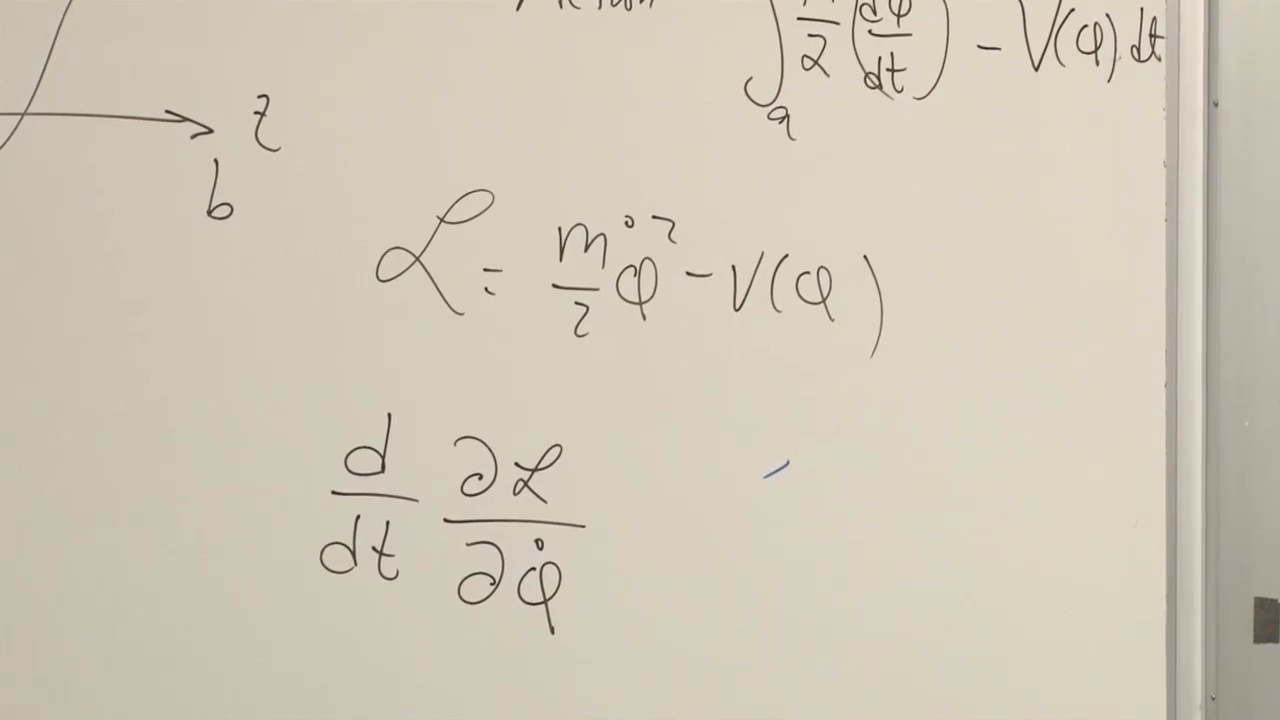
\includegraphics[width=0.90\textwidth]{lecture_04_figure_02.png}
\caption{Lịch sử được lấy mẫu \(\phi(t)\): một quỹ đạo hạt và, với một cách diễn giải mới, một lịch sử trường trong \(0+1\) chiều.}
\lectureframe{00:14:30}
\end{figure}

\begin{classroomqa}
\audiencequestion{Thế năng có biến mất khi không có chiều không gian nào không?}
\lecturerresponse{Không. Sự biến thiên theo không gian biến mất, nhưng trường vẫn có một giá trị. Năng lượng có thể phụ thuộc vào giá trị đó thông qua \(V(\phi)\). Trong cách diễn giải hạt, dịch đường cong lên hoặc xuống làm thay đổi thế năng; trong cách diễn giải trường, các giá trị khác nhau của \(\phi\) mang những thế năng khác nhau. \lecturetimestamp{00:15:00}}
\end{classroomqa}

\begin{classroomqa}
\audiencequestion{Thay vì tưởng tượng hoàn toàn không có không gian, có thể tưởng tượng một không gian thông thường mà trong đó trường chỉ phụ thuộc vào thời gian không?}
\lecturerresponse{Có. Với mục đích này, toán học cục bộ là như nhau: mọi đạo hàm theo không gian đều triệt tiêu và chỉ còn \(\phi(t)\). Gọi đó là một lý thuyết \(0+1\) chiều giúp tách riêng cấu trúc rút gọn ấy, nhưng một trường đồng nhất theo không gian trong một thế giới lớn hơn cũng cho cùng một trực giác. \lecturetimestamp{00:16:25}}
\end{classroomqa}

Mục đích của sự đi đường vòng này giờ đã rõ. Ta biết nguyên lý tác dụng cho một trường phụ thuộc vào một tọa độ, là thời gian. Ta có thể dùng khuôn mẫu đó để đoán nguyên lý tác dụng cho một trường phụ thuộc vào tất cả các tọa độ của không-thời gian.

\section{Lịch sử trường trên không-thời gian}

\subsection{Từ một đường cong đến một mặt}

Trong \(1+1\) chiều, bản thân không-thời gian là một mặt phẳng với các tọa độ \(t\) và \(x\). Giá trị \(\phi(x,t)\) cung cấp một hướng thứ ba. Vì vậy, lịch sử của trường không còn là một đường cong mà là một mặt nằm phía trên mặt phẳng không-thời gian. Mặt đó có thể vươn lên trên hoặc hạ xuống dưới không, vì một trường vô hướng không nhất thiết phải dương.

\begin{figure}[htbp]
\centering
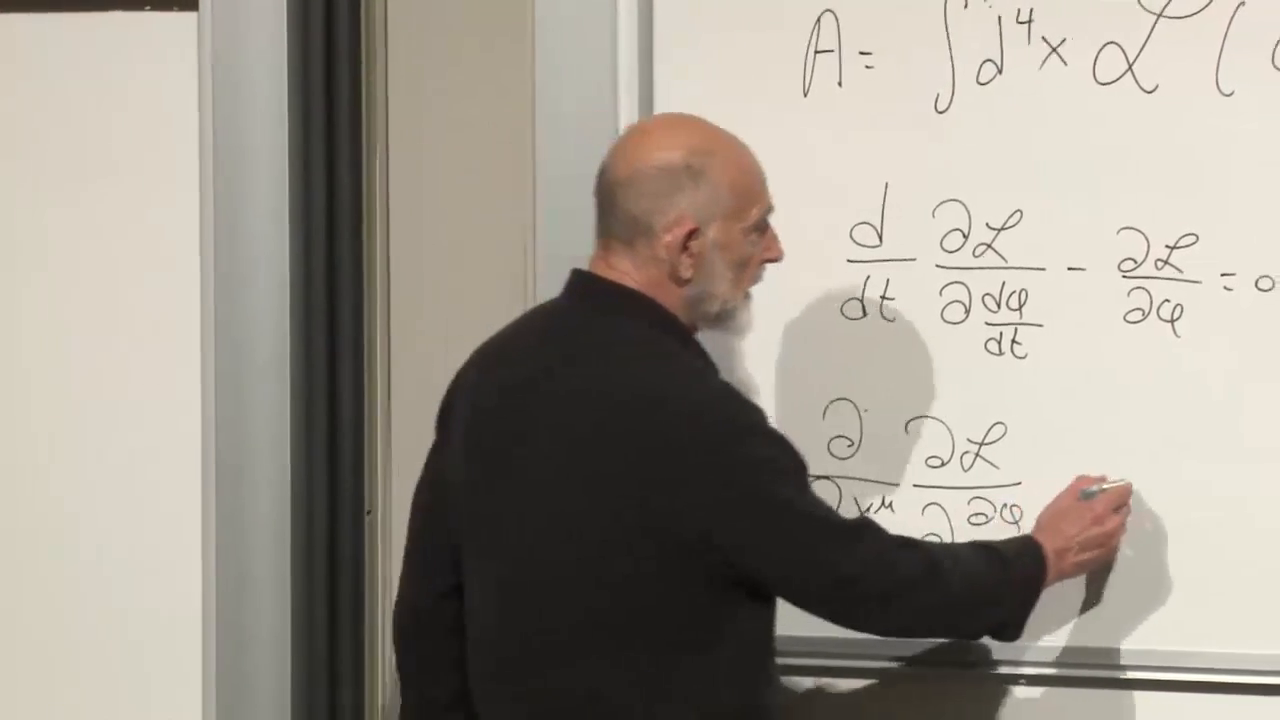
\includegraphics[width=0.90\textwidth]{lecture_04_figure_03.png}
\caption{Lịch sử của một trường vô hướng được vẽ như một mặt trên một mặt phẳng không-thời gian \(1+1\) chiều.}
\lectureframe{00:20:46}
\end{figure}

Không-thời gian vật lý của chúng ta được gọi là \(3+1\) chiều: ba chiều không gian và một chiều thời gian. Một mô hình trên mặt bàn có \(2+1\) chiều, và các hạt bị ràng buộc trên một sợi dây gợi ra một thế giới \(1+1\) chiều. Trục phụ thêm cần để biểu diễn \(\phi\) khiến ngay cả trường hợp \(3+1\) cũng không thể được vẽ một cách trung thực, nhưng định nghĩa thì không mơ hồ: một lịch sử đầy đủ gán một giá trị của \(\phi\) cho mọi sự kiện không-thời gian.

\subsection{Từ các đầu mút cố định đến dữ liệu biên cố định}

Bài toán biến phân của hạt giữ cố định hai đầu mút và biến thiên đường cong giữa chúng. Phép tương tự trong lý thuyết trường chọn một miền không-thời gian, giữ cố định \(\phi\) trên biên của miền đó, và biến thiên \(\phi\) ở bên trong. Miền ấy có thể là một hình chữ nhật trong hình vẽ \(1+1\) chiều hoặc bất kỳ miền thích hợp nào trong một không-thời gian nhiều chiều hơn.

\begin{figure}[htbp]
\centering
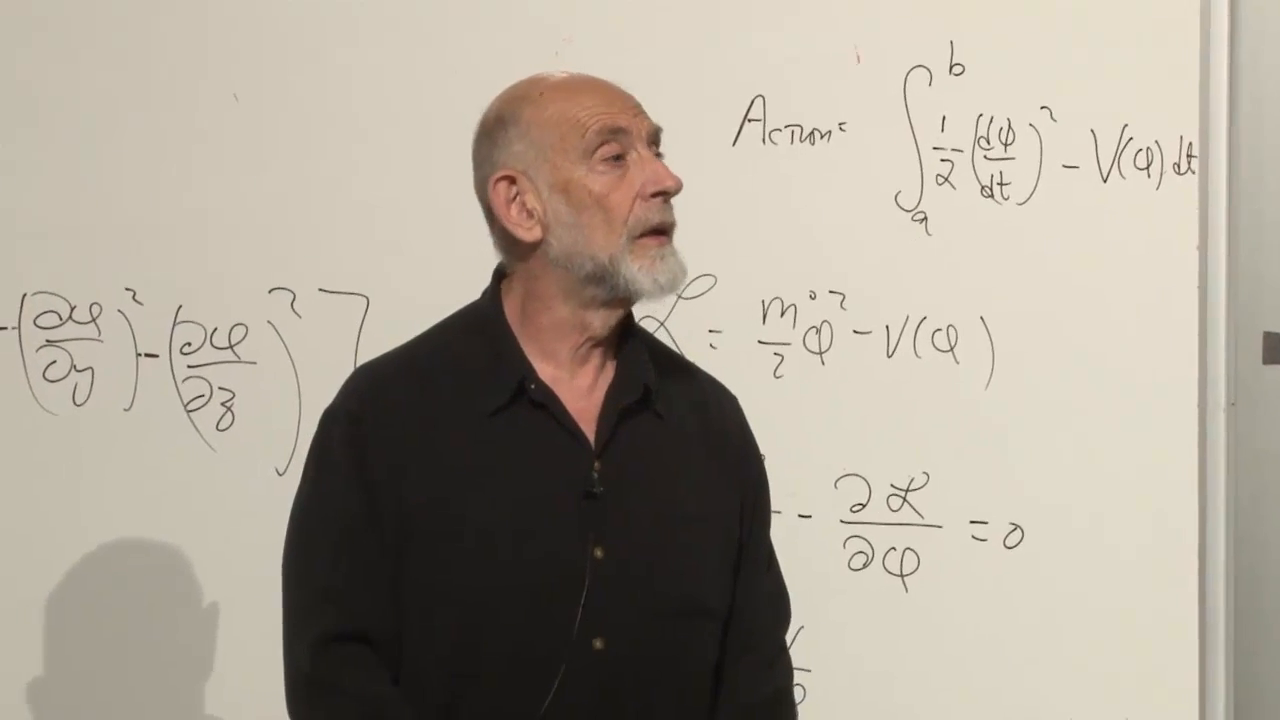
\includegraphics[width=0.90\textwidth]{lecture_04_figure_04.png}
\caption{Một miền không-thời gian mà toàn bộ biên của nó được giữ cố định, trong khi trường ở bên trong được biến thiên.}
\lectureframe{00:24:52}
\end{figure}

\begin{classroomqa}
\audiencequestion{Khuôn khổ Lagrangian có còn hoạt động khi một thế năng phụ thuộc tường minh vào thời gian không?}
\lecturerresponse{Có. Các khuôn khổ Euler--Lagrange và Hamilton vẫn hoạt động. Điều mất đi, nói chung, là sự bảo toàn năng lượng: sự phụ thuộc tường minh vào thời gian phá vỡ đối xứng tịnh tiến theo thời gian. Phát biểu tương ứng trong lý thuyết trường là sự phụ thuộc tường minh vào không-thời gian được cho phép, mặc dù nó ảnh hưởng đến các định luật bảo toàn liên hệ. \lecturetimestamp{00:23:49}}
\end{classroomqa}

\begin{classroomqa}
\audiencequestion{Đối với miền trường hình chữ nhật, chỉ phần trên và dưới được giữ cố định, hay là toàn bộ biên?}
\lecturerresponse{Đối với cấu trúc biến phân này, toàn bộ biên được giữ cố định: cả bốn cạnh của hình chữ nhật \(1+1\) chiều. Trường chỉ được phép dao động ở bên trong. Đây là phép tương tự trực tiếp của việc giữ cố định cả hai đầu mút trong cơ học hạt. \lecturetimestamp{00:24:24}}
\end{classroomqa}

Việc cố định toàn bộ biên là một phát biểu về phép biến phân dùng để suy ra các phương trình. Khi phương trình trường siêubol thu được được xem như một bài toán tiến hóa vật lý, người ta thường sẽ chỉ định dữ liệu đầu thích hợp và để phương trình truyền nó về phía trước.

\section{Tác dụng và phương trình Euler--Lagrange của trường}

\subsection{Mật độ Lagrangian}

Hãy chia miền không-thời gian thành các ô nhỏ. Tác dụng được giả định là tổng của các đóng góp địa phương, mỗi ô một đóng góp. Trong giới hạn liên tục, tổng đó trở thành một tích phân trên không-thời gian:
\begin{equation}
A[\phi]
=
\int_{\Omega} d^4x\,
\mathcal{L}\!\left(
\phi,\partial_\mu\phi;x^\mu
\right),
\qquad
d^4x=dt\,dx\,dy\,dz.
\label{eq:sr4-field-action}
\end{equation}
Đại lượng \(\mathcal{L}\) là mật độ Lagrangian. Dấu chấm phẩy trong \(\mathcal{L}(\phi,\partial_\mu\phi;x^\mu)\) tách các đối số động lực học khỏi sự phụ thuộc tường minh có thể có vào tọa độ. Trong một hệ kín đồng nhất, sự phụ thuộc sau cùng đó thường không có, nhưng hình thức luận biến phân không cấm nó.

Ký hiệu gọn
\begin{equation}
\partial_\mu\phi
\equiv
\frac{\partial\phi}{\partial x^\mu}
\end{equation}
gom các đạo hàm theo thời gian và không gian lại với nhau. Trong ký hiệu theo thành phần của bài giảng, thay vào đó có thể viết
\begin{equation}
\begin{aligned}
\phi_t&=\frac{\partial\phi}{\partial t},\\
\phi_x&=\frac{\partial\phi}{\partial x},\\
\phi_y&=\frac{\partial\phi}{\partial y},\\
\phi_z&=\frac{\partial\phi}{\partial z}.
\end{aligned}
\label{eq:sr4-component-derivatives}
\end{equation}
Có thể có nhiều trường, cũng như một hạt có thể có nhiều tọa độ. Hiện tại chỉ có một trường \(\phi\).

Ký hiệu \(d^4x\) chỉ là viết tắt cho phần tử đo bốn tọa độ. Trong một không-thời gian có số chiều khác, nó sẽ được thay bằng \(d^Dx\). Trong nguyên mẫu \(0+1\) chiều, \(D=1\) và \(d^1x\) đơn giản là \(dt\).

\begin{figure}[htbp]
\centering
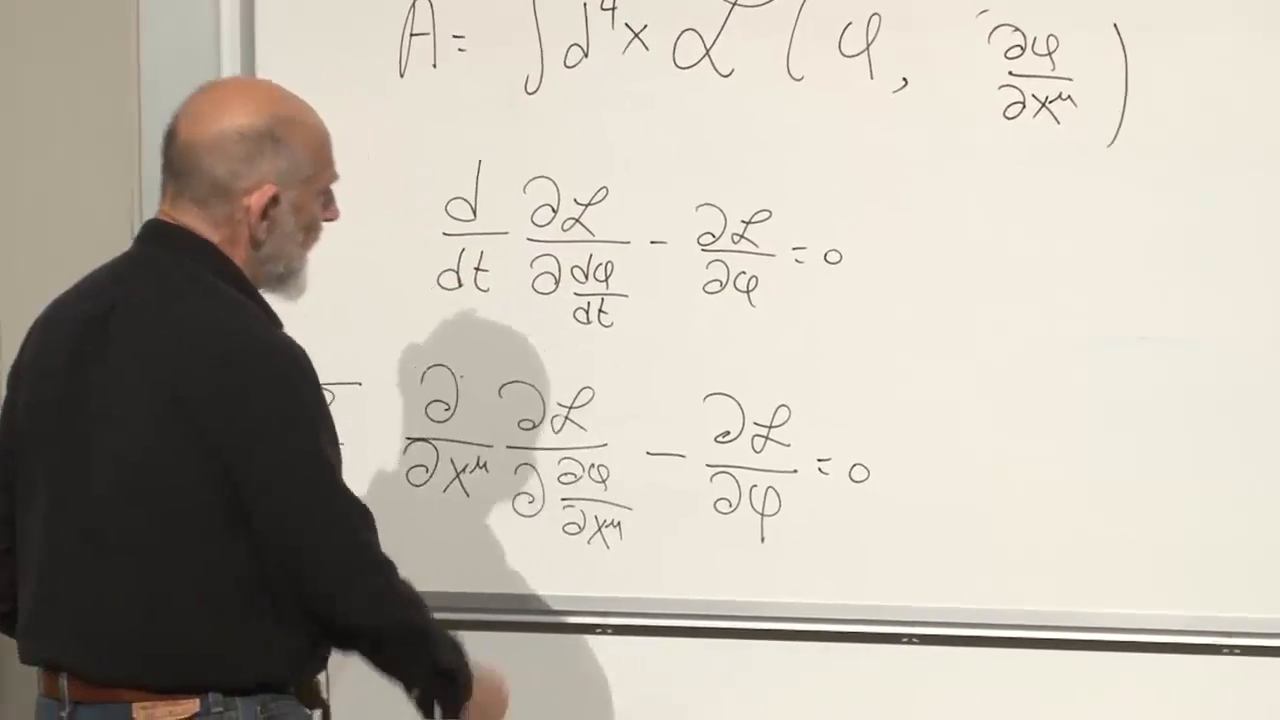
\includegraphics[width=0.90\textwidth]{lecture_04_figure_05.png}
\caption{Mật độ tác dụng được viết như một hàm địa phương của \(\phi\) và các đạo hàm không-thời gian của nó.}
\lectureframe{00:32:51}
\end{figure}

\begin{classroomqa}
\audiencequestion{Mật độ Lagrangian có thể cũng phụ thuộc vào chính \(x,y,z\) không?}
\lecturerresponse{Có thể, cũng như Lagrangian của hạt có thể phụ thuộc tường minh vào \(t\). Đối với một hệ kín bất biến đối với tịnh tiến, thông thường nó không như vậy, nhưng sự phụ thuộc tường minh vào tọa độ không làm mất hiệu lực của hình thức luận. \lecturetimestamp{00:30:29}}
\end{classroomqa}

\begin{classroomqa}
\audiencequestion{Cho đến đây, sự xây dựng này dành riêng cho một trường vô hướng, hay là tổng quát?}
\lecturerresponse{Cho đến đây, mô thức biến phân là tổng quát. Việc chỉ viết một thành phần gợi ý một trường vô hướng. Một trường vectơ hoặc một tập các trường sẽ mang thêm các nhãn thành phần, và ta sẽ biến phân theo mọi thành phần. \lecturetimestamp{00:31:00}}
\end{classroomqa}

\subsection{Bức tranh mạng lưới}

Trên một mạng không-thời gian đủ mịn, các đạo hàm trở thành các sai phân hữu hạn giữa những giá trị trường lân cận. Khi đó tác dụng là một hàm thông thường của nhiều biến. Một lưới có mười điểm theo một hướng và tám theo hướng kia đã cho tám mươi biến trường. Làm mịn lưới hơn sẽ làm tăng số lượng của chúng, nhưng quy tắc cực tiểu hóa vẫn sơ đẳng: lấy đạo hàm của tác dụng theo giá trị trường tại mỗi điểm bên trong và cho kết quả bằng không.

\begin{figure}[htbp]
\centering
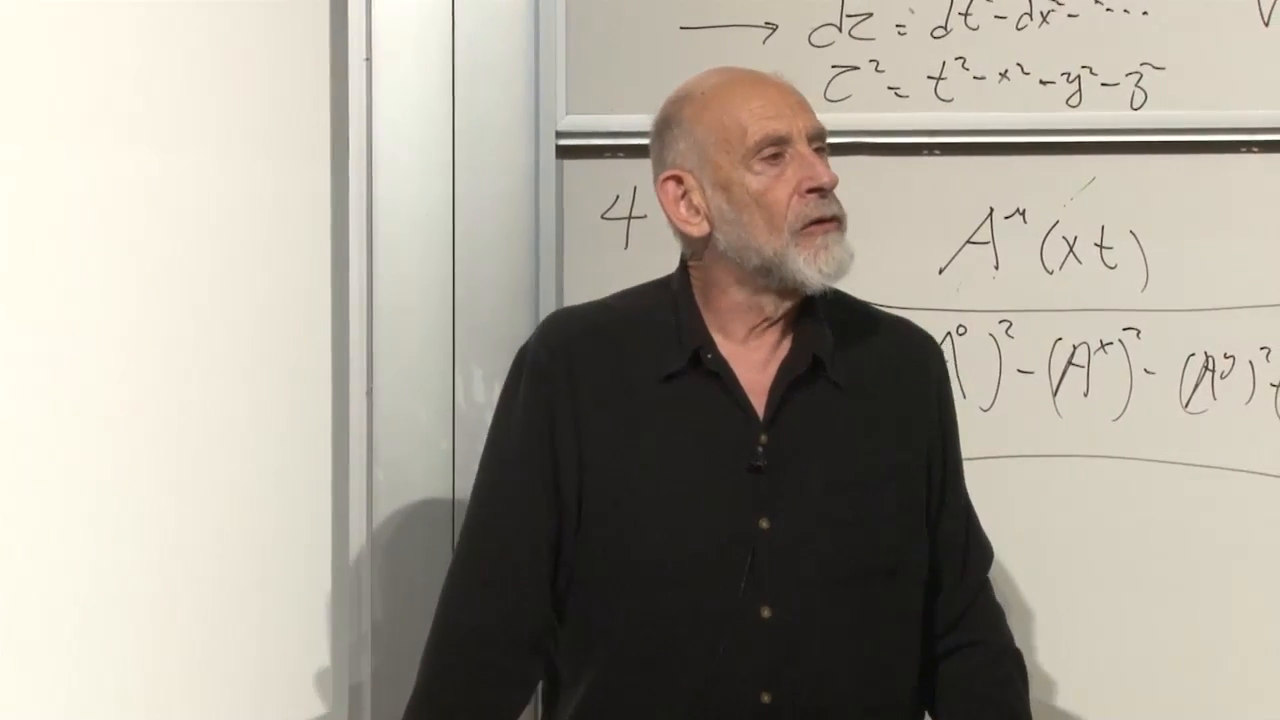
\includegraphics[width=0.90\textwidth]{lecture_04_figure_06.png}
\caption{Miền không-thời gian được chia thành các ô, khiến tác dụng trở thành một hàm nhiều biến thông thường trước khi lấy giới hạn liên tục.}
\lectureframe{00:34:05}
\end{figure}

Lấy giới hạn liên tục cho ta phương trình Euler--Lagrange của trường,
\begin{equation}
\boxed{
\partial_\mu
\left[
\frac{\partial\mathcal{L}}
{\partial(\partial_\mu\phi)}
\right]
-
\frac{\partial\mathcal{L}}{\partial\phi}
=0
}.
\label{eq:sr4-field-el}
\end{equation}
Khi \(\mu\) lặp lại, ta ngầm cộng trên mọi hướng không-thời gian. Viết ra mà không dùng ký hiệu tắt của phép tổng, cùng phương trình ấy là
\begin{align}
&
\frac{\partial}{\partial t}
\left(\frac{\partial\mathcal{L}}{\partial\phi_t}\right)
+
\frac{\partial}{\partial x}
\left(\frac{\partial\mathcal{L}}{\partial\phi_x}\right)
+
\frac{\partial}{\partial y}
\left(\frac{\partial\mathcal{L}}{\partial\phi_y}\right)
\nonumber\\
&\hspace{3em}
+
\frac{\partial}{\partial z}
\left(\frac{\partial\mathcal{L}}{\partial\phi_z}\right)
-
\frac{\partial\mathcal{L}}{\partial\phi}
=0.
\label{eq:sr4-field-el-expanded}
\end{align}
Hạng đầu tiên là hạng quen thuộc của hạt. Lý thuyết trường thêm một hạng tương tự cho mỗi hướng không gian. Hạng cuối cùng, \(-\partial\mathcal{L}/\partial\phi\), không đổi.

\begin{figure}[htbp]
\centering
\includegraphics[width=0.90\textwidth]{lecture_04_figure_07.png}
\caption{Phương trình Euler--Lagrange một chiều và tổng quát hóa không-thời gian của nó, được viết cái nọ bên dưới cái kia.}
\lectureframe{00:38:44}
\end{figure}

Chủ đề này cũng được gọi là cơ học liên tục. Tùy theo các bậc tự do, cùng một toán học có thể mô tả dòng chảy chất lưu, chuyển vị đàn hồi, hoặc một môi trường liên tục khác.

\begin{classroomqa}
\audiencequestion{Những phương trình đó có còn dùng được trong một thế giới có không gian mà không có thời gian không?}
\lecturerresponse{Có, dưới dạng một bài toán biến phân thuần túy theo không gian. Về mặt vật lý, đó là cách người ta tìm một nghiệm tĩnh: giả sử trường không phụ thuộc thời gian, bỏ mọi đạo hàm theo thời gian, rồi giải các phương trình không gian còn lại. Một cấu hình điện trường hoặc từ trường không phụ thuộc thời gian là một ví dụ. \lecturetimestamp{00:40:05}}
\end{classroomqa}

\section{Phỏng đoán dạng động lực học vô hướng đơn giản nhất}

\subsection{Vì sao các dấu không thể đều giống nhau}

Quay lại hạng động năng của hạt \(\tfrac12\dot\phi^2\), đặt hệ số tổng thể không quan trọng của nó bằng một, rồi thử khái quát hóa nó. Một dự đoán đầu tiên có thể là
\begin{equation}
\mathcal{L}_{+}
=
\frac12
\left[
\phi_t^2+\phi_x^2+\phi_y^2+\phi_z^2
\right].
\label{eq:sr4-all-plus}
\end{equation}
Đây là một ngã rẽ sai nhưng hữu ích. Nó xử lý thời gian và không gian với các dấu giống hệt nhau. Phương trình thu được sẽ không có cấu trúc hyperbolic của sự truyền sóng. Tổ hợp tương đối tính đúng dùng một dấu cho thời gian và dấu ngược lại cho không gian.

\begin{classroomqa}
\audiencequestion{Biểu thức toàn dấu cộng có sai vì Lagrangian phải bất biến tương đối tính không?}
\lecturerresponse{Đó là câu trả lời sâu hơn, và nó đúng. Bài giảng trước hết đi tới dấu đó theo một cách sơ khai hơn: sóng phân biệt sự tiến hóa theo thời gian với sự biến thiên theo không gian, nên thời gian không thể đi vào đúng hệt như một tọa độ không gian khác. Tính bất biến Lorentz sẽ sớm biến trực giác ấy thành một quy tắc chính xác. \lecturetimestamp{00:43:19}}
\end{classroomqa}

Khôi phục một tốc độ đặc trưng \(c\), ta có mật độ Lagrangian vô hướng đơn giản
\begin{equation}
\boxed{
\mathcal{L}
=
\frac12
\left[
\frac{1}{c^2}\phi_t^2
-\phi_x^2-\phi_y^2-\phi_z^2
\right]
-V(\phi)
}.
\label{eq:sr4-scalar-lagrangian}
\end{equation}
Đối với một trường tương đối tính, \(c\) là tốc độ ánh sáng. Trong một mô hình môi trường liên tục, thay vào đó nó có thể là tốc độ âm thanh, tốc độ của sóng đàn hồi, hoặc một tốc độ truyền đặc trưng khác.

Hệ số tổng thể \(1/2\) chỉ là quy ước, cũng như trong
\(\tfrac12m\dot\phi^2\). Nhân toàn bộ tác dụng với một hằng số khác không không làm thay đổi các quỹ đạo dừng của nó; quy ước này cố định cách đặt tên và chuẩn hóa các tham số trong các phương trình. Một khi đã chọn chuẩn hóa đó, phải dùng nó một cách nhất quán.

\begin{classroomqa}
\audiencequestion{Có thể xem các hạng gradient không gian là một phần của thế năng không?}
\lecturerresponse{Có. Trong cách sắp xếp kiểu động năng trừ thế năng, phần động năng chứa các đạo hàm theo thời gian. Các hạng không chứa đạo hàm theo thời gian, bao gồm các gradient không gian và \(V(\phi)\), thuộc về phía thế năng. Lý do cuối cùng của dấu tương đối giữa chúng trong một lý thuyết tương đối tính là metric Lorentzian. \lecturetimestamp{00:45:37}}
\end{classroomqa}

\subsection{Phương trình sóng}

Áp dụng \eqref{eq:sr4-field-el}. Các hạng đạo hàm là
\begin{equation}
\frac{\partial\mathcal{L}}{\partial\phi_t}
=\frac{1}{c^2}\phi_t,
\qquad
\frac{\partial\mathcal{L}}{\partial\phi_i}
=-\phi_i,
\end{equation}
trong khi
\begin{equation}
\frac{\partial\mathcal{L}}{\partial\phi}
=-\frac{dV}{d\phi}.
\end{equation}
Vì vậy
\begin{equation}
\begin{aligned}
&\boxed{
\frac{1}{c^2}\frac{\partial^2\phi}{\partial t^2}
-\nabla^2\phi
+\frac{dV}{d\phi}
=0
},\\[0.5em]
\nabla^2
&=
\frac{\partial^2}{\partial x^2}
+\frac{\partial^2}{\partial y^2}\\
&\quad
+\frac{\partial^2}{\partial z^2}.
\end{aligned}
\label{eq:sr4-general-scalar-eom}
\end{equation}

Nếu \(V=0\), phương trình này rút gọn thành
\begin{equation}
\boxed{
\frac{1}{c^2}\phi_{tt}-\nabla^2\phi=0
},
\label{eq:sr4-wave-equation}
\end{equation}
chính là phương trình sóng. Bài giảng nhận ra phương trình này nhưng hoãn việc giải nó lại. Các nghiệm của nó truyền nhiễu loạn với tốc độ \(c\).

\begin{figure}[htbp]
\centering
\includegraphics[width=0.90\textwidth]{lecture_04_figure_08.png}
\caption{Dạng một chiều \(c^{-2}\phi_{tt}-\phi_{xx}=0\), được nhận ra là phương trình sóng.}
\lectureframe{00:50:30}
\end{figure}

\subsection{Một trường gồm các dao động điều hòa ghép}

Giờ hãy chọn một thế năng bậc hai,
\begin{equation}
V(\phi)=\frac12\mu^2\phi^2,
\qquad
\frac{dV}{d\phi}=\mu^2\phi.
\label{eq:sr4-quadratic-potential}
\end{equation}
Nếu \(\phi\) là tọa độ của một hạt, thì đây sẽ là thế năng của một dao động tử điều hòa có hằng số lò xo \(\mu^2\). Đối với trường,
\begin{equation}
\boxed{
\frac{1}{c^2}\phi_{tt}-\nabla^2\phi+\mu^2\phi=0
}.
\label{eq:sr4-klein-gordon}
\end{equation}
Nếu bỏ đạo hàm không gian đi, thì đây đơn giản là gia tốc cộng một hằng số nhân độ dời bằng không. Gradient ghép các điểm lân cận với nhau, biến dao động tử thành một môi trường liên tục mang sóng. Trong lý thuyết trường tương đối tính, \eqref{eq:sr4-klein-gordon} được gọi là phương trình Klein--Gordon có khối lượng; về mặt cổ điển, \(\mu\) là thang độ dài nghịch đảo làm biến đổi sự truyền sóng.

\begin{figure}[htbp]
\centering
\includegraphics[width=0.90\textwidth]{lecture_04_figure_09.png}
\caption{Thế năng bậc hai và phương trình sóng thu được với hạng hồi phục \(\mu^2\phi\).}
\lectureframe{00:52:38}
\end{figure}

\begin{classroomqa}
\audiencequestion{Vì sao hệ số \(1/2\) trong \(V=\tfrac12\mu^2\phi^2\) lại biến mất khỏi phương trình chuyển động?}
\lecturerresponse{Lấy đạo hàm của \(\phi^2\) tạo ra một hệ số hai. \(1/2\) theo quy ước được đưa vào chính xác để \(dV/d\phi=\mu^2\phi\), đúng như \(V(x)=\tfrac12kx^2\) cho lực hồi phục \(-kx\). \lecturetimestamp{00:53:17}}
\end{classroomqa}

Phương trình là tuyến tính: \(\phi\) và mỗi đạo hàm của nó đều chỉ xuất hiện ở lũy thừa bậc nhất. Các hạng như \(\phi^2\) hoặc \(\phi\,\partial_\mu\phi\) trong phương trình chuyển động sẽ làm cho động lực học trở nên phi tuyến.

\section{Vô hướng Lorentz và bốn-vectơ}

\subsection{Tác dụng phải độc lập với hệ quy chiếu}

Chỉ riêng bộ máy biến phân đã xác định được nhiều lý thuyết trường khả dĩ. Thuyết tương đối áp đặt thêm yêu cầu rằng tác dụng phải có cùng giá trị và cùng dạng trong mọi hệ quy chiếu quán tính. Với hạt tự do, điều này đạt được bằng cách lấy tích phân thời gian riêng bất biến \(d\tau\) dọc theo đường thế. Với một trường, tác dụng được lấy tích phân trên không-thời gian, nên các thành phần cục bộ cấu thành nó phải biến đổi một cách thích hợp.

Dưới một phép biến đổi Lorentz proper, độ đo không-thời gian là bất biến,
\(d^4x'=d^4x\). Vì thế, chỉ cần yêu cầu mật độ Lagrangian là một vô hướng Lorentz:
\begin{equation}
\mathcal{L}'(x')=\mathcal{L}(x).
\label{eq:sr4-lagrangian-scalar}
\end{equation}

\subsection{Trường vô hướng}

Một trường vô hướng tuân theo
\begin{equation}
\boxed{\phi'(x')=\phi(x)}.
\label{eq:sr4-scalar-transform}
\end{equation}
Các tọa độ \(x\) và \(x'\) gắn nhãn cho cùng một sự kiện trong hai hệ quy chiếu. Các biểu thức hàm mà những người quan sát dùng có thể trông khác nhau, nhưng giá trị số gắn với sự kiện vật lý đó là như nhau.

\begin{figure}[htbp]
\centering
\includegraphics[width=0.90\textwidth]{lecture_04_figure_10.png}
\caption{Định luật biến đổi định nghĩa của một trường vô hướng: \(\phi(x)=\phi'(x')\).}
\lectureframe{00:59:33}
\end{figure}

Nhiệt độ đã đem lại trực giác ban đầu, mặc dù một nhiệt kế đang chuyển động trong một môi trường vật chất không phải là ví dụ tương đối tính hoàn hảo. Điều quan trọng là định nghĩa
\eqref{eq:sr4-scalar-transform}, chứ không phải phép loại suy bằng nhiệt kế.

\subsection{Bốn-vectơ}

Trong đơn vị \(c=1\), một phép boost với tốc độ \(v\) dọc theo trục \(x\) có dạng
\begin{equation}
\begin{aligned}
t'&=\gamma(t-vx),\\
x'&=\gamma(x-vt),\\
y'&=y,\\
z'&=z,\\
\gamma&=\frac{1}{\sqrt{1-v^2}}.
\end{aligned}
\label{eq:sr4-x-boost}
\end{equation}

\begin{figure}[htbp]
\centering
\includegraphics[width=0.90\textwidth]{lecture_04_figure_11.png}
\caption{Phép biến đổi Lorentz cho một phép boost dọc theo trục \(x\) trong đơn vị \(c=1\).}
\lectureframe{01:02:26}
\end{figure}

Bất kỳ bốn đại lượng nào trộn lẫn với nhau dưới các phép boost theo cùng một cách đều tạo thành một bốn-vectơ. Các ví dụ đã gặp là \(x^\mu\), \(dx^\mu\), và bốn-vận tốc \(u^\mu=dx^\mu/d\tau\). Nhân một bốn-vectơ với một vô hướng cho ra một bốn-vectơ khác. Một chất lưu tương đối tính đang chảy cho một ví dụ kiểu trường: bốn-vận tốc của nó \(u^\mu(x)\) có thể khác nhau từ sự kiện này sang sự kiện khác.

Đối với cùng phép boost như trong \eqref{eq:sr4-x-boost}, một bốn-vectơ tổng quát tuân theo
\begin{equation}
\begin{aligned}
A'^0&=\gamma(A^0-vA^x),\\
A'^x&=\gamma(A^x-vA^0),\\
A'^y&=A^y,\\
A'^z&=A^z.
\end{aligned}
\label{eq:sr4-vector-boost}
\end{equation}

Đối với một bốn-vectơ tổng quát \(A^\mu=(A^0,A^x,A^y,A^z)\), chuẩn Lorentz
\begin{equation}
\boxed{
A_\mu A^\mu
=(A^0)^2-(A^x)^2-(A^y)^2-(A^z)^2
}
\label{eq:sr4-vector-norm}
\end{equation}
là một vô hướng. Nó là bất biến vì cùng một lý do đại số khiến
\begin{equation}
d\tau^2=dt^2-dx^2-dy^2-dz^2
\end{equation}
là bất biến. Bài giảng thoáng chốc hết các chữ cái chưa dùng cho một vectơ tổng quát trước khi chấp nhận \(A\), nhờ gợi ý \(A\) cho arrow.

\begin{figure}[htbp]
\centering
\includegraphics[width=0.90\textwidth]{lecture_04_figure_12.png}
\caption{Một trường bốn-vectơ tổng quát và hiệu bình phương kiểu Lorentz dùng để tạo ra chuẩn bất biến của nó.}
\lectureframe{01:09:06}
\end{figure}

\subsection{Đạo hàm của một vô hướng}

Lấy đạo hàm một vô hướng theo bốn tọa độ không-thời gian cho ra bốn thành phần
\begin{equation}
\partial_\mu\phi
=
\left(
\frac{\partial\phi}{\partial t},
\frac{\partial\phi}{\partial x},
\frac{\partial\phi}{\partial y},
\frac{\partial\phi}{\partial z}
\right)
\qquad(c=1).
\end{equation}
Nói chặt chẽ hơn, \(\partial_\mu\phi\) là một đối vectơ; metric Minkowski nâng chỉ số của nó lên để tạo thành \(\partial^\mu\phi\). Sự phân biệt này là vô hại trong lập luận theo thành phần ở đây, nhưng nó xác định phép co chỉ số một cách không mơ hồ:
\begin{equation}
\boxed{
\partial_\mu\phi\,\partial^\mu\phi
=
\frac{1}{c^2}\phi_t^2
-\phi_x^2-\phi_y^2-\phi_z^2
}.
\label{eq:sr4-derivative-scalar}
\end{equation}

\begin{figure}[htbp]
\centering
\includegraphics[width=0.90\textwidth]{lecture_04_figure_13.png}
\caption{Hiệu bình phương bất biến được xây dựng từ các đạo hàm bậc nhất của một trường vô hướng.}
\lectureframe{01:13:55}
\end{figure}

\begin{classroomqa}
\audiencequestion{Tổ hợp đạo hàm này có phải là Laplacian không?}
\lecturerresponse{Không. Bất biến được hiển thị là bậc hai theo các đạo hàm bậc nhất. Laplacian chứa các đạo hàm không gian bậc hai. Các đạo hàm bậc hai chỉ xuất hiện sau khi lấy biến phân của tác dụng, trong phương trình sóng. \lecturetimestamp{01:13:22}}
\end{classroomqa}

Mẫu dấu trong \eqref{eq:sr4-scalar-lagrangian} nay đã được giải thích thay vì chỉ phỏng đoán. Tổ hợp giữa hạng động năng và hạng gradient là vô hướng Lorentz
\(\partial_\mu\phi\,\partial^\mu\phi\). Vì thế, lý thuyết bậc hai đơn giản nhất là
\begin{equation}
\mathcal{L}
=
\frac12\partial_\mu\phi\,\partial^\mu\phi
-\frac12\mu^2\phi^2.
\label{eq:sr4-covariant-lagrangian}
\end{equation}

\begin{figure}[htbp]
\centering
\includegraphics[width=0.90\textwidth]{lecture_04_figure_14.png}
\caption{Mật độ Lagrangian hoàn chỉnh của trường vô hướng bậc hai và phương trình trường tuyến tính của nó trên bảng.}
\lectureframe{01:19:12}
\end{figure}

\section{Có bao nhiêu tự do lựa chọn?}

Một khi đã biết quy tắc để xây dựng các vô hướng, nhiều Lagrangian trở nên khả dĩ. Trường \(\phi\) là một vô hướng, nên mọi hàm thông thường \(F(\phi)\) cũng là một vô hướng: \(\phi^2\), \(\phi^3\), \(\cosh\phi\), v.v. Các tham số số cũng được phép. Có thể chèn một ký hiệu như \(\mu\) làm hệ số hằng; những câu hỏi còn lại duy nhất là thứ nguyên của nó và cách diễn giải vật lý của nó.

\begin{classroomqa}
\audiencequestion{Có thể đưa khối lượng vào Lagrangian không?}
\lecturerresponse{Một tham số hằng thì chắc chắn có thể. Ở giai đoạn này nên hỏi đó là khối lượng của đối tượng nào, vì \(\mu\) chỉ đơn thuần là một con số trong lý thuyết trường cổ điển cho đến khi ý nghĩa vật lý của nó được xác định. Trong lý thuyết vô hướng tương đối tính bậc hai, nó ấn định khối lượng hoặc thang độ dài nghịch đảo. \lecturetimestamp{01:14:16}}
\end{classroomqa}

Các vô hướng có thể được nhân với nhau:
\begin{equation}
F(\phi)\,\partial_\mu\phi\,\partial^\mu\phi
\end{equation}
là bất biến Lorentz. Chính vô hướng đạo hàm đó cũng có thể được bình phương, tạo ra các lũy thừa cao hơn của các đạo hàm bậc nhất. Ta cũng có thể xét các đạo hàm bậc cao hơn, mặc dù bài giảng chỉ giới hạn ở các trường và các đạo hàm bậc nhất của chúng, khuôn khổ tiêu chuẩn cho ra các phương trình chuyển động bậc hai. Các lý thuyết có đạo hàm bậc cao đòi hỏi sự thận trọng bổ sung vì nói chung chúng đưa vào dữ liệu động lực học phụ thêm và những bất ổn khả dĩ.

\begin{classroomqa}
\audiencequestion{Cấu trúc hiệu các bình phương này thực sự có phải là metric của không-thời gian không?}
\lecturerresponse{Đúng. Metric trong quy ước dấu đã chọn là \(dt^2-dx^2-dy^2-dz^2\). Bài giảng chưa nhấn mạnh từ metric, nhưng đây chính là hình học không-thời gian sẽ trở thành trung tâm của thuyết tương đối rộng. \lecturetimestamp{01:19:39}}
\end{classroomqa}

\begin{classroomqa}
\audiencequestion{Có những đối tượng tổng quát hơn bốn-vectơ không, với các thành phần như \(xy\) hoặc \(tx\)?}
\lecturerresponse{Có. Đó là các tensor. Một vô hướng không có chỉ số không-thời gian, một vectơ có một chỉ số, và một tensor hạng hai có các thành phần như \(T^{xx}\), \(T^{xy}\), và \(T^{tx}\). Phần lớn thảo luận hiện tại về trường vô hướng tránh chúng; chúng trở nên không thể né tránh trong thuyết tương đối rộng. \lecturetimestamp{01:20:49}}
\end{classroomqa}

\begin{classroomqa}
\audiencequestion{Vì sao chỉ thảo luận các phép boost trộn \(t\) với \(x\)? Một phép boost có thể hướng theo phương khác và trộn các trục không gian theo cách khác không?}
\lecturerresponse{Dĩ nhiên. Một phép boost dọc theo \(y\) trộn \(t\) với \(y\) và để \(x,z\) không đổi. Một phép biến đổi Lorentz tổng quát có thể được ghép từ các phép quay không gian và một phép boost dọc theo một trục đã chọn. Vì vậy, chỉ cần thiết lập tính bất biến quay và tính bất biến dưới một phép boost theo một trục chuẩn. \lecturetimestamp{01:22:06}}
\end{classroomqa}

\begin{classroomqa}
\audiencequestion{Với quá nhiều tổ hợp vô hướng có thể có như vậy, phải chăng mọi Lagrangian thu được đều mô tả vật lý có ý nghĩa?}
\lecturerresponse{Ở mức cổ điển, sự tự do là vô cùng lớn, nhưng vẫn chịu các yêu cầu bổ sung như dấu hợp lý, tính địa phương và một bài toán tiến hóa đặt chỉnh. Có ít lựa chọn tùy ý hơn nhiều mới xác định được các lý thuyết lượng tử cơ bản ứng xử tốt. Lý thuyết trường hiệu dụng hiện đại cho phép nhiều tương tác bổ sung dưới một thang cắt, nhưng khi đó phải nêu rõ miền hiệu lực của chúng. \lecturetimestamp{01:27:57}}
\end{classroomqa}

\begin{classroomqa}
\audiencequestion{Một trường có nhất thiết phải liên tục không?}
\lecturerresponse{Đối với các lý thuyết trơn đang được thảo luận, có. Một chỗ nhảy tạo ra các đạo hàm kỳ dị và, với một hạng gradient bậc hai, thường dẫn tới tác dụng và năng lượng vô hạn. Những cấu hình kỳ dị hơn chỉ có thể được xử lý khi có thêm cấu trúc toán học; chúng không phải là các trường năng lượng hữu hạn thông thường đang được xây dựng ở đây. \lecturetimestamp{01:29:29}}
\end{classroomqa}

\section{Một hạt ghép với một trường vô hướng}

\subsection{Xét lại hạt tự do}

Phần cuối của bài giảng kết nối các hạt và các trường ở mức cổ điển. Đây vẫn chưa phải là phát biểu lượng tử rằng các hạt là những kích thích của trường. Thay vào đó, giả sử ai đó đã xác định được một trường vô hướng nền \(\phi(x,t)\), rồi hỏi một hạt chuyển động trong đó như thế nào.

Đối với một hạt tương đối tính tự do,
\begin{equation}
A_{\rm free}=-m\int d\tau.
\label{eq:sr4-free-particle-action}
\end{equation}
Trong một chiều không gian và \(c=1\),
\begin{equation}
d\tau=dt\sqrt{1-\dot x^2},
\qquad
L_{\rm free}=-m\sqrt{1-\dot x^2}.
\label{eq:sr4-free-particle-l}
\end{equation}
Dấu trừ được chọn để khai triển theo vận tốc nhỏ cho ra hạng động năng Newton quen thuộc với dấu dương:
\begin{equation}
L_{\rm free}
\approx -m+\frac12m\dot x^2+\cdots.
\end{equation}

\begin{figure}[htbp]
\centering
\includegraphics[width=0.90\textwidth]{lecture_04_figure_15.png}
\caption{Hàm tác dụng bất biến của hạt tự do được viết lại dưới dạng Lagrangian theo thời gian tọa độ.}
\lectureframe{01:34:31}
\end{figure}

\subsection{Ghép cặp vô hướng đơn giản nhất}

Cả \(d\tau\) lẫn \(\phi\) đều là vô hướng. Vì vậy ghép cặp tuyến tính đơn giản nhất là
\begin{equation}
\boxed{
A
=
\int d\tau\,[-m+\phi(x,t)]
}.
\label{eq:sr4-coupled-action}
\end{equation}
Lựa chọn này không phải là duy nhất. Có thể thay \(\phi\) bằng một hàm bất kỳ \(F(\phi)\). Hạng tuyến tính là đủ để làm rõ ý tưởng vật lý.

\begin{figure}[htbp]
\centering
\includegraphics[width=0.90\textwidth]{lecture_04_figure_16.png}
\caption{Hàm tác dụng tự do được bổ sung thêm ghép cặp vô hướng bất biến Lorentz đơn giản nhất.}
\lectureframe{01:37:21}
\end{figure}

\begin{classroomqa}
\audiencequestion{Liệu \(\phi\) có phải vẫn nằm bên trong dấu tích phân không?}
\lecturerresponse{Có. Trường được lấy giá trị trên đường thế giới của hạt, \(\phi(x(t),t)\), và nói chung thay đổi từ điểm này của quỹ đạo sang điểm khác. Ngay cả khi trường nền không có phụ thuộc tường minh vào thời gian, \(\phi=\phi(x)\), giá trị của nó vẫn thay đổi theo thời gian khi hạt chuyển động trong không gian. Chỉ một trường không đổi dọc theo đường đi mới có thể được đưa ra ngoài. \lecturetimestamp{01:37:47}}
\end{classroomqa}

\begin{classroomqa}
\audiencequestion{Liệu \(x\) trong \(\phi(x,t)\) có nghĩa là vị trí của hạt không?}
\lecturerresponse{Vâng. Nó là \(x=x(t)\), vị trí của hạt tại thời điểm \(t\). Hàm tác dụng lấy giá trị của trường không-thời gian đã cho dọc theo quỹ đạo đó. \lecturetimestamp{01:38:08}}
\end{classroomqa}

Đối với chuyển động một chiều, \eqref{eq:sr4-coupled-action} cho
\begin{equation}
L
=
-(m-\phi(x,t))\sqrt{1-\dot x^2}.
\label{eq:sr4-coupled-lagrangian}
\end{equation}
Trường nền vô hướng xuất hiện đúng ở vị trí mà khối lượng nghỉ chiếm:
\begin{equation}
m_{\rm eff}(x,t)=m-\phi(x,t).
\label{eq:sr4-effective-mass}
\end{equation}
Nếu \(\phi\) ổn định ở một giá trị gần như hằng khác không, hạt ứng xử như thể khối lượng của nó đã bị dịch chuyển. Đây chỉ là một mô hình đồ chơi cổ điển, không phải cơ chế Higgs đầy đủ, nhưng nó nắm được đúng cái hương vị đã được báo trước của ý tưởng Higgs: một nền vô hướng có thể đi vào động lực học của hạt như một hạng khối lượng.

\subsection{Phương trình của hạt}

Xung lượng chính tắc là
\begin{equation}
p
=
\frac{\partial L}{\partial\dot x}
=
(m-\phi)
\frac{\dot x}{\sqrt{1-\dot x^2}}.
\label{eq:sr4-coupled-momentum}
\end{equation}

\begin{figure}[htbp]
\centering
\includegraphics[width=0.90\textwidth]{lecture_04_figure_17.png}
\caption{Nền vô hướng thay \(m\) bằng \(m-\phi(x,t)\) trong xung lượng chính tắc tương đối tính.}
\lectureframe{01:43:38}
\end{figure}

Đạo hàm theo vị trí của Lagrangian là
\begin{equation}
\frac{\partial L}{\partial x}
=
\frac{\partial\phi}{\partial x}
\sqrt{1-\dot x^2}.
\end{equation}
Giữ dấu như được cố định bởi hàm tác dụng
\eqref{eq:sr4-coupled-action}, phương trình Euler--Lagrange do đó là
\begin{equation}
\boxed{
\frac{d}{dt}
\left[
(m-\phi)
\frac{\dot x}{\sqrt{1-\dot x^2}}
\right]
=
\frac{\partial\phi}{\partial x}
\sqrt{1-\dot x^2}
}.
\label{eq:sr4-coupled-eom}
\end{equation}

\begin{figure}[htbp]
\centering
\includegraphics[width=0.90\textwidth]{lecture_04_figure_18.png}
\caption{Phương trình ghép cặp được dựng từ xung lượng và đạo hàm theo không gian của trường nền; hàm tác dụng cố định dấu cuối cùng trong \eqref{eq:sr4-coupled-eom}.}
\lectureframe{01:45:24}
\end{figure}

\begin{classroomqa}
\audiencequestion{Tại sao \(\partial\phi/\partial x\) vẫn giữ thừa số \(\sqrt{1-\dot x^2}\)?}
\lecturerresponse{Vì chỉ thừa số \(\phi(x,t)\) được lấy đạo hàm theo \(x\). Căn bậc hai nhân với nó trong Lagrangian và độc lập với vị trí khi \(\dot x\) được giữ cố định trong đạo hàm riêng, nên căn bậc hai vẫn còn. \lecturetimestamp{01:45:50}}
\end{classroomqa}

Khai triển đạo hàm toàn phần theo thời gian ta được
\begin{align}
&(m-\phi)
\frac{d}{dt}
\left(
\frac{\dot x}{\sqrt{1-\dot x^2}}
\right)
-
\dot\phi\,
\frac{\dot x}{\sqrt{1-\dot x^2}}
\nonumber\\
&\hspace{10em}
=
\frac{\partial\phi}{\partial x}
\sqrt{1-\dot x^2}.
\label{eq:sr4-coupled-expanded}
\end{align}
Nếu trường nền là tĩnh, \(\phi=\phi(x)\), thì đạo hàm của nó dọc theo đường thế giới của hạt đang chuyển động không bằng 0. Quy tắc dây chuyền cho
\begin{equation}
\boxed{
\dot\phi
=
\frac{d}{dt}\phi(x(t))
=
\frac{\partial\phi}{\partial x}\dot x
}.
\label{eq:sr4-chain-rule}
\end{equation}

\begin{classroomqa}
\audiencequestion{Nếu \(\phi\) không có phụ thuộc tường minh vào thời gian, tại sao \(\dot\phi\) lại không bằng 0?}
\lecturerresponse{Vì hạt thay đổi vị trí. Trường được lấy giá trị tại \(x(t)\), nên đạo hàm toàn phần của nó là \(\dot\phi=\phi_x\dot x\). Trường tĩnh có nghĩa là \(\partial\phi/\partial t=0\), chứ không phải mọi hạt đang chuyển động đều thấy một giá trị trường không đổi. \lecturetimestamp{01:48:10}}
\end{classroomqa}

\begin{figure}[htbp]
\centering
\includegraphics[width=0.90\textwidth]{lecture_04_figure_19.png}
\caption{Bước khai triển tiếp theo của phương trình ghép cặp sau khi dùng quy tắc dây chuyền dọc theo đường thế giới.}
\lectureframe{01:49:11}
\end{figure}

Biểu thức chính xác không đặc biệt gọn đẹp, và bài giảng cũng không hề vờ như khác đi. Tuy vậy, giới hạn vận tốc chậm của nó vẫn quen thuộc. Vì \(\sqrt{1-\dot x^2}\approx1\), phương trình bậc dẫn là
\begin{equation}
\frac{d}{dt}\bigl[(m-\phi)\dot x\bigr]
\approx
\frac{\partial\phi}{\partial x}.
\end{equation}
Nếu sự biến thiên của khối lượng hiệu dụng cũng được xử lý theo nhiễu loạn, thì phương trình này thành
\begin{equation}
(m-\phi)\ddot x
\approx
\frac{\partial\phi}{\partial x}.
\label{eq:sr4-nonrel-force}
\end{equation}
Thật vậy, Lagrangian ở vận tốc thấp là
\begin{equation}
L
\approx
-m+\phi+\frac12(m-\phi)\dot x^2,
\end{equation}
nên ở bậc dẫn thế năng là \(U=-\phi\) và lực là
\(-dU/dx=\partial_x\phi\). Khôi phục các thừa số của \(c\) và thu lại dạng thức Newton này là bài tập khép lại bài giảng.

Con đường từ hạt đến trường giờ đã hoàn tất. Một lịch sử hạt \(\phi(t)\) đã cung cấp nguyên mẫu \(0+1\)-chiều; một lịch sử trường \(\phi(x)\) đã nâng hàm tác dụng thành một tích phân trên không-thời gian; phương trình Euler--Lagrange của trường đã sinh ra động lực học sóng; các vô hướng Lorentz đã chọn ra cấu trúc dấu tương đối tính; và cùng ngôn ngữ bất biến ấy đã cho phép một nền vô hướng tác động ngược trở lại lên một hạt.